\documentclass[a4paper,twoside,titlepage, openright, 11pt]{report}
\usepackage[ngerman]{babel}
%\usepackage[ansinew]{inputenc}
\usepackage[ansinew]{inputenc}
\usepackage[numbers,square]{natbib}
\usepackage{graphicx}
\usepackage{fancyhdr}
\usepackage{capt-of}
\usepackage{setspace}
\usepackage[font=bf]{caption}
\usepackage{chngcntr}
%\usepackage[hidelinks]{hyperref}
\usepackage{listings}
\usepackage{color}
\usepackage{amsmath}
\usepackage[T1]{fontenc}
%\usepackage[bottom=4cm]{geometry}

%\usepackage[automark]{scrpage2}
\newcommand{\changefont}[3]{
\fontfamily{#1} \fontseries{#2} \fontshape{#3} \selectfont}


\DeclareCaptionFont{white}{\color{white}}
\DeclareCaptionFormat{listing}{\colorbox{white}{\parbox{\textwidth}{#1#2#3}}}
\captionsetup[lstlisting]{format=listing,labelfont=white,textfont=white}
\definecolor{dkgreen}{rgb}{0,0.8,0}
\definecolor{gray}{rgb}{0.95,0.95,0.95}
\definecolor{mauve}{rgb}{0.58,0,0.82}


\lstset{
  language=C++,                % choose the language of the code
  basicstyle=\tiny\ttfamily, 
  numbers=left,                   % where to put the line-numbers
  stepnumber=1,                   % the step between two line-numbers.        
  numbersep=4pt,                  % how far the line-numbers are from the code
  backgroundcolor=\color{gray},   % choose the background color. You must add \usepackage{color}
  showspaces=false,               % show spaces adding particular underscores
  showstringspaces=false,         % underline spaces within strings
  showtabs=false,                 % show tabs within strings adding particular underscores
  tabsize=2,                      % sets default tabsize to 2 spaces
  captionpos=t,                   % sets the caption-position to bottom
  breaklines=false,               % sets automatic line breaking
  breakatwhitespace=true,         % sets if automatic breaks should only happen at whitespace
  xleftmargin=4pt,
 % title=\lstname,                % show the filename of files included with \lstinputlisting;
  keywordstyle=\color{blue},      % keyword style
  commentstyle=\color{dkgreen},   % comment style
  stringstyle=\color{mauve},      % string literal style
}


\counterwithin{figure}{chapter}
\onehalfspacing
\setlength{\headheight}{15pt}

\newcommand{\blankpage}{
\newpage
\thispagestyle{empty}
\mbox{}
\newpage
}
 
 \raggedbottom
\begin{document}


%\changefont{ptm}{m}{n}
\nocite{*}
\bibliographystyle{plain}
\renewcommand{\thepage}{\Roman{page}}
\setcounter{secnumdepth}{-2}

\thispagestyle{empty}
\begin{titlepage}
	\begin{flushleft}
			Bauhaus-Universit�t Weimar\\
			Fakult�t Medien\\
			Studiengang Mediensysteme
	\end{flushleft}
	\begin{verbatim}





	\end{verbatim}
	\begin{center}
		\Large \textbf{Erstellung, Segmentierung und Out-Of-Core Speichermanagement von Sparse Voxel Octrees}
	\end{center}
	\begin{verbatim}





	\end{verbatim}
	\begin{center}
		\Large Diplomarbeit
	\end{center}
	\begin{verbatim}



	\end{verbatim}
	\begin{center}
		Felix Wei�ig\\
		Matrikelnummer: ------\\
		geb. am 10.10.1979 in Hoyerswerda\\
	\begin{verbatim}



	\end{verbatim}
		1. Gutachter: Prof. Dr. Charles A. W�thrich\\
		%2. Gutachter: Prof. Dr. Guido Morgenthal \,\,\,

	\begin{verbatim}



	\end{verbatim}
	Datum der Abgabe: xx. M�rz 2013
	\end{center}

	
\end{titlepage}

\blankpage
\section{Erkl�rung}

Hiermit versichere ich, dass ich die vorliegende Diplomarbeit selbstst�ndig angefertigt, 
anderweitig nicht f�r Pr�fungszwecke vorgelegt und alle verwendeten Quellen angegeben habe.
\begin{verbatim}




\end{verbatim}
Felix Wei�ig
\begin{verbatim}



\end{verbatim}
Weimar, den 25. M�rz 2013

\blankpage
\section{Danksagung}
An dieser Stelle m�chte ich mich zun�chst bei Prof. Dr. Charles W�thrich f�r die Annahme und Bewertung meiner Diplomarbeit bedanken. Ein Dank geht auch an Bernhard Bittorf, dessen moralische Unterst�tzung mir w�hrend des Entstehens der Arbeit sehr geholfen hat. Ein gro�er Dank geht vor allem an Henning Gr�ndl, Sebastian Thiele, Konstantin Silin und Stephan Beck f�r lebhafte Diskussionen und Hilfe bei der Bearbeitung des schriftlichen Teils dieser Arbeit. Benjamin Bendig muss im Besonderen f�r seine hervorragende Arbeit bei der Implementation des in dieser Arbeit verwendeten OpenCL-Wrappers \textit{benCL} erw�hnt werden. Kaum genug danken kann ich meinen Eltern f�r die jahrelange Unterst�tzung w�hrend meines ausschweifenden Studiums.\\
Der gr��te Dank geht jedoch an meine Freundin und Lebensgef�hrtin Eva Johanna M�hlemann, die mir in den zur�ckliegenden Monaten den R�cken frei hielt und mir dadurch den Freiraum gab diese Arbeit zu bew�ltigen.

Danke.  

\blankpage
\section{Kurzfassung}

Voxel+Ray=Pixel
\blankpage
\addtocontents{toc}{\protect\thispagestyle{empty}}
\tableofcontents
\thispagestyle{empty}
\listoffigures
\blankpage
\thispagestyle{empty}
\renewcommand{\thepage}{\arabic{page}}
\setcounter{secnumdepth}{2}


%\pagestyle{scrheadings} 
%\clearscrheadfoot 
%\ihead{\headmark} 
%\ohead{Name} 
%\renewcommand*{\chapterpagestyle}{chapter}

\newpage
\renewcommand{\sectionmark}[1]{}
\setcounter{page}{1}

\fancyhf{} % clear all header and footer fields
%\fancyfoot[C]{\thepage} % except the center
%\fancyhead[EL]{\nouppercase{\leftmark}}
%\fancyhead[OL]{\nouppercase{\rightmark}}


\fancyfoot[LE,RO]{\thepage}
\pagestyle{fancy}
\fancyhead[LE,RO]{\slshape \rightmark}
\fancyhead[LO,RE]{\slshape \leftmark}
%\renewcommand{\chaptermark}[1]{\markboth{\thechapter.\space#1}{}}

\renewcommand{\chaptermark}[1]{\markright{#1}{}}
  \makeatletter
 \let\ps@plain\ps@fancy
 \makeatother
\chapter{Einleitung}
\section{Motivation}
Seit langer Zeit ist die Bild\-synthese durch Ras\-teris\-ierung von pa\-rame\-tri\-sierten Dreiecken der Quasi-Standard f�r Echtzeitcomputergrafik. Diese Entwicklung wurde nicht zuletzt durch die Einf�hrung von dedizierter Hardware und offenen Standards, wie OpenGL m�glich. Der Vorteil von Dreiecken als Geometrieprimitiv ist, dass sich mit ihnen sehr effizient planare Fl�chen darstellen lassen. Dabei hat die Gr��e der abgebildeten Fl�chen keinen Einfluss auf den Speicherbedarf der Repr�sentation. In modernen Anwendungen wie Spielen oder bei der Darstellung von hochaufl�senden 3D-Scanns ist dieser Vorteil jedoch immer weniger relevant da der �berwiegende Teil des ben�tigten Speichers durch Texturen belegt wird. Diese werden ben�tigt um die Fl�chen mit Details zu versehen, wie Farbe, Richtung und anderen zur Beleuchtung ben�tigten Attributen. Dabei ist die Parametrisierung von komplex geformten Dreiecksnetzen mit Textur\-koordinaten nicht trivial und muss meist von Hand bewerkstelligt werden.\\
Bei der Rasterisierung von detaillierten Dreiecksnetzen mit hochaufgel�sten Texturen kommt es zu Ali\-asing\-artefakten. Um diese zu reduzieren werden von Dreiecks\-netzen und Texturen niedriger aufgel�ste, sta\-tische Versionen erzeugt (\textit{Level-of-Detail, LOD}). Zwischen diesen Versionen wird bei der Darstellung je nach Betrachtungsabstand gewechselt, was zu st�renden \textit{Popping}-Artifakten f�hrt wenn eine LOD-Stufe durch eine andere ausgetauscht wird. Mit dieser Technik kann nur selten ein ideales Verh�ltnis zwischen Geometrie- und Bildaufl�sung gew�hrleistet werden. Dynamische Erzeugung von LOD-Stufen ist mit hohem Rechen- oder Speicheraufwand verbunden. Au�erdem muss das LOD-Problem f�r Geometrie- und Texturdaten w�hrend der Erstellung und der Darstellung separat gel�st werden. Ein Nachteil des Rasterisierungsansatzes ist das Fehlen von globalen Informationen w�hrend der Fragmentgenerierung. Jedes Primitiv wird f�r sich behandelt, ohne dass globale Informationen zur Optimierung (\textit{Culling}) oder Beleuchtung (\textit{Global Illumination}) zur Verf�gung stehen.
\begin{figure}[position=h]
  \centering
  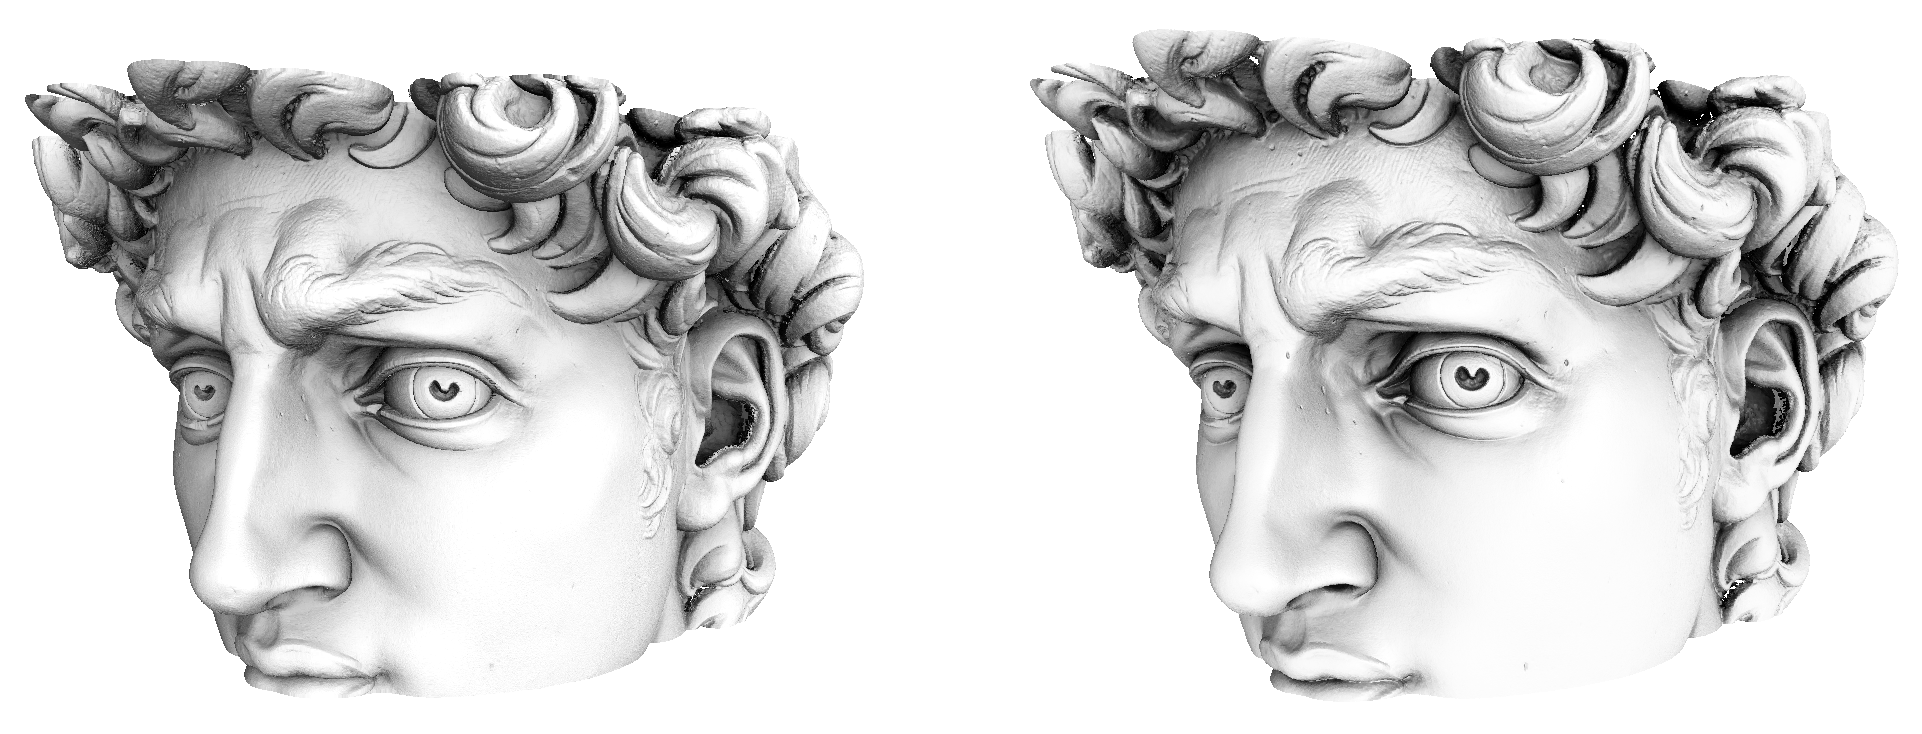
\includegraphics[width=1.0\textwidth]{figures/mesh_and_svo.png}
  \caption{Darstellung von Dreicksnetz und Sparse Voxel Octree \label{mesh_and_svo}}
\end{figure}
Die Generalisierung der Renderpipelines und die Einf�hrung von GPGPU-Hochsprachen wie OpenCL machen es m�glich, die Frage nach geeigneten Geometrieprimitiven und Bildsyntheseverfahren neu zu stellen. Sparse Voxel Octree (SVO) als Datenstruktur in Kombination mit \textit{Raycasting} als Algorithmus zur Bildsynthese bieten viele positive Eigenschaften. Sparse Voxel Octrees vereinen Geometrie- und Texturdaten in einer gemeinsamen hierarchischen Datenstruktur. Durch Raycasting auf dieser Struktur kann das LOD-Problem f�r Geometrie- und Texturdaten gleichzeitig pro Bildpunkt gel�st werden. Der Octree wirkt dabei als eine Beschleunigungs\-struktur, so dass w�hrend des Traversierens nur die Teile der Struktur durchlaufen werden, die zur Bildsynthese beitragen. Eine Parametrisierung ist nicht notwendig da jedes Voxel seine ei\-genen Attributinformationen spei\-chert die f�r seine Gr��e in optimaler Aufl�sung vorliegen. Abbildung \ref{mesh_and_svo} zeigt die Darstellung eines Modells als Dreiecksnetz (linkes Bild) und als Sparse Voxel Octree (rechtes Bild).\\
Dennoch gibt es einige Herausforderungen die vor der Verwendung von Sparse Voxe Octrees bew�ltigt werden m�ssen. Sparse Voxel Octrees ben�tigen viel Speicher. Die Menge an Arbeitsspeicher aktueller Grafikkarten ist f�r einige Anwendungen ausreichend, um SVO-Strukturen in hinreichend hoher Aufl�sung zu speichern. Ben�tigt man jedoch h�here Aufl�sung, um m�glichst viele Details beziehungsweise sehr gro�e Strukturen abbilden zu k�nnen, fallen schnell mehrere Gigabyte an Daten an, die dann nicht mehr als Ganzes in den GPU-Speicher passen.
Da Sparse Voxel Octrees erst in j�ngster Zeit in den Fokus von Wissenschaft und Industrie ger�ckt sind, sind sie in Programmen zur Erstellung von 3D-Inhalten noch nicht angekommen. Daher ist es zun�chst notwendig Sparse Voxel Octrees aus anderen Geometrie\-repr�sentationen zu erstellen. Dreicksnetze, Punktwolken, H�henfelder oder Volumendaten k�nnen als Eingabedaten dienen. Um unterschiedliche Repr�sentationen von Inhalten ohne gro�en Ent\-wicklungs\-aufwand unterst�tzen zu k�nnen fehlt ein generisches System das diese Daten verarbeiten kann.


\section{Zielstellung}
Ziel dieser Arbeit soll die Entwicklung eines Out-Of-Core Ansatzes sein, der basierend auf Segmentierung der Daten eine adaptive Verfeinerung der Darstellung erm�glicht. Um dies zu unterst�tzen soll au�erdem ein generisches Systems zur Erstellung von SVO-Strukturen aus unterschiedlichen Eingabedaten wie Dreiecksnetzen, Punktwolken oder Volumendaten entwickelt werden. Die Bildgenerierung soll durch Raycasting auf den erzeugten Sparse-Voxel-Octree-Strukturen erm�glicht werden. Die n�tigen Berechnungen sollen auf aktueller Grafik-Hardware ausgef�hrt werden um interaktive Bild\-wiederhol\-raten zu erreichen.

%\newpage
\chapter{Verwendete Infrastruktur}


\section{gloost framework}
gloost ist ..


\section{bencl-OpenCl Wrapper}
bencl ist ...
%\newpage
\chapter{Grundlagen}


\section{Volumendaten}
Volumendaten k�nnen durch dreidimensionale, �quidistante Gitter beschrieben werden. Die Kreuzungspunkte des Gitters werden \textit Voxel (Volumen-Pixel) genannt. Jeder Voxel kann einen einzelnen skalaren Wert, wie beispielsweise Dichte oder Druck, oder mehrere skalare Werte wie Farbe in Kombination mit Richtungsinformationen enthalten. Dadurch eignet sich diese Darstellung zur Repr�sentation eines �quidistant gesampelten Raumes, der nicht homogen gef�llt ist. Durch die uniforme Unterteilung des Raumes ist die Position und die Ausdehnung eines jeden Voxels implizit in der Datenstruktur enthalten und muss daher nicht gespeichert werden.\\
Volumendaten werden vorwiegend in der Medizin, beispielsweise als Ausgabe der Magnetresonanztomographie oder in der Geologie zum Abbilden der Ergebnisse von Reflexionsseismikverfahren verwendet.\\
Um eine hinreichende Aufl�sung der Volumenrepr�sentation zu gew�hrleisten sind gro�e Datenmengen erforderlich. Ein mit $512^3$ Voxeln aufgel�stes Volumen, dessen Voxel jeweils einen mit 4 Byte abgebildeten Skalar enthalten, belegt bereits 512 Megabyte. Verdoppelt man die Aufl�sung auf $1024^3$ verachtfacht sich der Speicherbedarf auf 4 Gigabyte. Allerdings enthalten Volumendaten in der Regel einen gro�en Anteil an homogenen Bereichen, die jedoch durch ein regul�res Gitter als viele Einzelwerte abgebildet werden m�ssen. Daher gibt es Datenstrukturen die ausgehend von dem regul�ren Gitter eine hierarchische Struktur erzeugen um diese Bereiche zusammenzufassen.


\section{Octrees}
Ein Octree ist eine raumteilende, rekursive Datenstruktur. Ein initiales, kubisches Volumen wird in acht gleich gro�e Untervolumen geteilt. Die Teilung wird f�r jedes Untervolumen fortgef�hrt, bis eine maximale Tiefe beziehungs\-weise ein maximaler Unterteilunggrad erreicht ist. Mit jeder Tiefen\-stufe des Octrees verdoppelt sich die Aufl�sung der abbildbaren Information auf jeder Achse. Die Gr��e eines Voxels kann mit $ 2^{-d} $ bestimmt werden wobei $d$ die Tiefe des Voxels in der Baumstruktur, beginnend mit $d=0$ f�r die Wurzel, ist. F�r vollbesetzte Octrees ist eine Darstellung im Speicher implizit vorgegeben. Da jeder Elternknoten genau acht Kinder besitzt kann durch seine Position in einer angenommenen, seriellen Struktur implizit auf seine Kind\-knoten geschlossen werden. Dabei kann die Position jedes Kindes eines Knotens durch $ C(P,n) = 8*P+n $ berechnet werden (!!!BILD) wobei $P$ die Position des Elternknotens, $n$ die Nummer des Kindes (beginnend mit 1) und das resultierende $C$ die Position des Kindknotens ist.\\
Bereiche, die homogene Daten enthalten oder leer sind, k�nnen jedoch von der Unterteilung ausgeschlossen werden, wodurch eine wesentlich kompaktere Darstellung der Daten gegen�ber konventionellen Volumendaten erreicht werden kann. F�r jedes Volumen/Voxel muss dann ein Verweis auf die ihn unterteilenden Untervolumen existieren. In der Regel besitzt jeder Voxel eines solchen Octrees acht Kinder (\textit{innerer Knoten}) oder kein Kind (\textit{Blatt-Knoten}). Die, im ung�nstigsten Fall zu speichernden sieben leeren Knoten, sind bei dieser Darstellung n�tig, um homogene Bereiche innerhalb des Eltern-Voxels zu kodieren.\\
Jeder Voxel kann ein oder mehrere Skalare speichern. Oft werden diese Werte nicht direkt im Octree abgelegt um bei die Traversierung der Struktur m�glichst wenig Speicher lesen zu m�ssen. Stattdessen werden die Attributinformation in einem zus�tzlichen Attribut-Buffer abgelegt, in dem zu jeder Voxel-Position im Octree ein Tuple mit Attributinformation an der selben Stelle im Attribut-Buffer vorgehalten wird. Die Attribute eines �bergeordneten Voxels ergeben sich dabei im einfachsten Fall aus dem Mittel der Attribute seiner untergeordneten Voxel, vergleichbar mit der Erzeugung von \textit{Mipmaps}. Somit enth�lt jeder Voxel einen seiner Gr��e entsprechend Detailgrad an Attributinformation. Der wesentliche Vorteil des Octrees gegen�ber texturierten Dreiecksnetzen ist somit, das die Datenstruktur das LOD-Problem nicht nur f�r Attribute (Texturen), sondern auch f�r Geometrie l�st. Der Octree ist also beides: Geometrie und Textur.


\section{Sparse Octrees}
F�r einige Anwendungen sind nur bestimmte Auspr�gungen der in den Voxeln gespeicherten Werte von Interesse. Beispielsweise werden beim Iso-Surface-Rendering nur Voxel mit einem bestimmten Dichtewert als opake Oberfl�che dargestellt. Ist dies der Fall kann die Datenstruktur weiter ausged�nnt werden, in dem nur noch Voxel gespeichert werden die zur Oberfl�che beitragen. Somit k�nnen innere Knoten weniger als acht Kinder haben. Eine solche ~Volumenrepr�sentation eignet sich ebenso zur Darstellung anderer opaker Oberfl�chen wie diskretisierte Dreiecksnetze, Punktwolken oder H�henfelder und wird als Sparse Octree oder Sparse Voxel Octree bezeichnet. Durch die variierende Anzahl von Kindknoten existiert keine implizite Regel zum berechnen deren Positionen. Vielmehr muss jeder Knoten speichern welche Kindknoten vorhanden sind und wo sich diese im Speicher befinden. Liegen die Kindknoten jedes Voxels jeweils hintereinander im Speicher muss nur ein Verweis pro Elternknoten vorgehalten werden.


\section{Raycasting}












%\newpage
\chapter{Out-Of-Core-Ansatz}

Out-of-Core-Strategien erm�glichen einer Anwendung oder einem System die Verwendung von Datenmengen, welche die lokale Speicherkapazit�t �bersteigen. Voraussetzung daf�r ist die Segmentierbarkeit der Daten. Ausserdem muss die lokal gespeicherte Untermenge der segmentierten Daten zu jedem Zeitpunkt zur Verarbeitung gen�gen.
\begin{figure}[position=h]
  \centering
  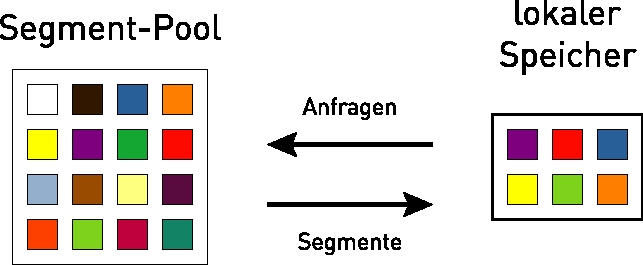
\includegraphics[width=0.75\textwidth]{out-of-core-ansatz/figures/out_of_core_pricipe.pdf}
  \caption{Out-Of-Core-Prinzip\label{out_of_core_pricipe}}
\end{figure}
\\
Die endliche Menge lokalen Speichers der GPU begrenzt die maximale Aufl�sungen der SVO-Struktur. Eine Vergr��erung des Speichers l�st das Problem nicht da wie oben beschrieben eine weitere SVO-Tiefe etwa die vierfache Speicher\-menge ben�tigt.


% /////////////////////////////////////////////////////////////////////////////

\section{Segmentierung}

Die Unterteilung der SVO-Struktur erfolgt in Unterb�umen fester Gr��e die in dieser Arbeit als \textit{Treelets} (B�umchen) bezeichnet werden. Ein Treelet hat eine eindeutige Kennung (\textit{Treelet-Id}) und h�lt unter Anderem Informationen �ber sein �bergeordnetes Treelet und seine untergeordneten Treeles wodurch eine zus�tzliche, bidirektionale Baumstruktur �ber dem eigentlichen Octree entsteht. Dabei entspricht jeder Blattknoten eines Eltern-Treelets dem Wurzelknoten eines Kind-Treelets.

\begin{figure}[position=h]
  \centering
  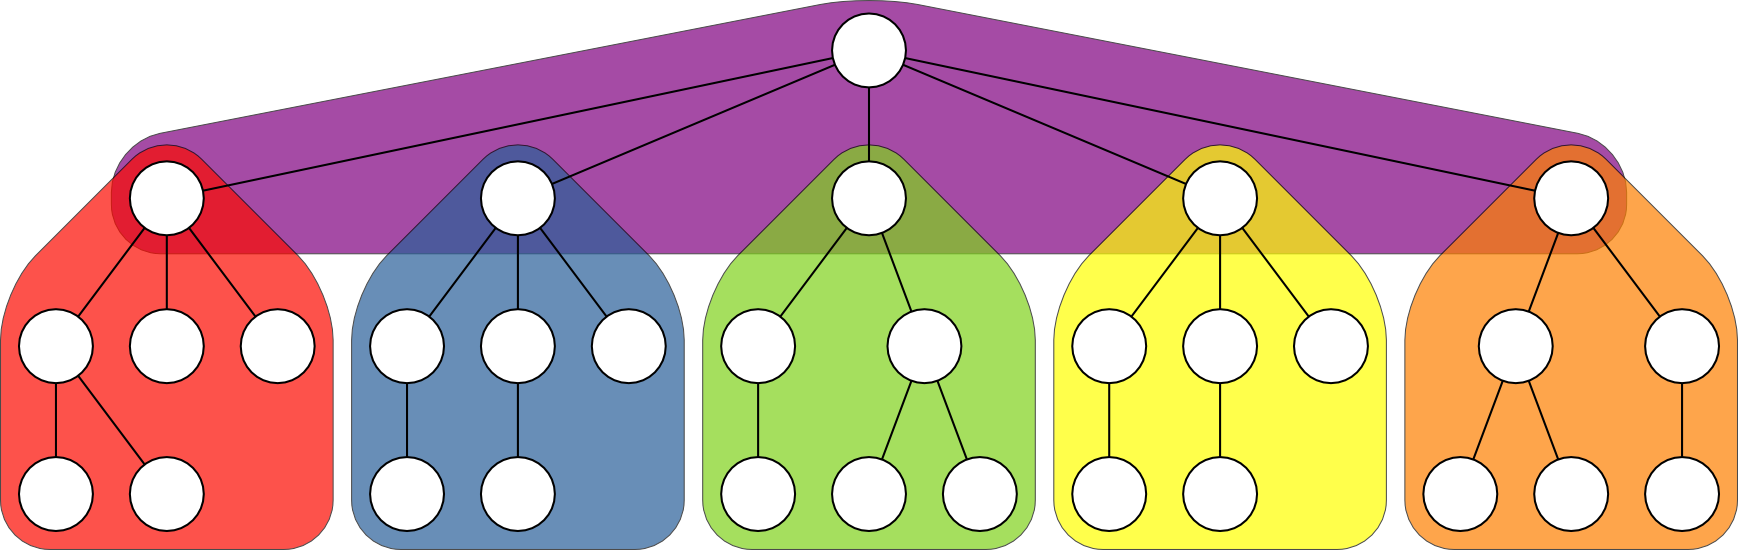
\includegraphics[width=0.75\textwidth]{out-of-core-ansatz/figures/fixed_size_treelets.pdf}
  \caption{Treelet-Struktur mit 6 Knoten pro Treelet \label{fixed_size_treelets}}
\end{figure}

Die Verbindung zum �bergeordneten Treelet (\textit{Eltern-Treelet}) ist wichtig, da aufgrund der zugrundeliegenden Baumstruktur die Verarbeitung eines Treelets das Vorhandensein des Eltern-Treelets voraussetzt. In jedem Treelet ist die Position des entsprechenden Blattknotens im Eltern-Treelet und die Position dessen Elternknoten gespeichert. Die Verbindungen nach unten sind im Erstes-Kind-Index der Blattknoten gespeichert, sind damit Teil der SVO-Daten und somit f�r alle Operationen auf auf dem SVO verf�gbar.\\
Die Speichergr��e eines Treelets ist variable und bewegt sich f�r die Tests in diese Arbeit zwischen einem und zehn Kilobyte. Um eine hohe Granularit�t und damit die M�glichkeit einer sehr feinen Anpassung der gew�hlten Untermenge an Segmenten zu gew�hrleisten sollte die Gr��e der Treelets eher klein gew�hlt werden. Sind die Treelets jedoch zu klein k�nnen f�r einen gegebenen Octree schnell mehrere Millionen Treelets entstehen, was das Out-Of-Core-System belastet. Deshalb ist es n�tig f�r jeden als Treelet-Struktur abzubildende Datensatz eine geeignete Treelet-G��e zu w�hlen.

!!! Verweis zu Untergeordneten Treelets in Blattknoten FirstChildIndex
 

% /////////////////////////////////////////////////////////////////////////////


\section{Prinzipieller Aufbau}

Der in dieser Arbeit verwendete Out-Of-Core-Ansatz besteht grunds�tzlich aus vier Teilen (Abbildung \ref{four_part_setup}): Einem gro�en, clientseitigem Buffer der die gesammte SVO-Struktur h�lt, einem vergleichsweise kleinen, serverseitigen Buffer der eine Untermenge der SVO-Struktur halten kann (\textbf{\textit{Incore-Buffer}}), einer Speicherverwaltung die den serverseitigen Buffer pflegt und einem Analysesystem das entscheidet welche Teile serverseitig ben�tigt werden.

\begin{figure}
  \centering
  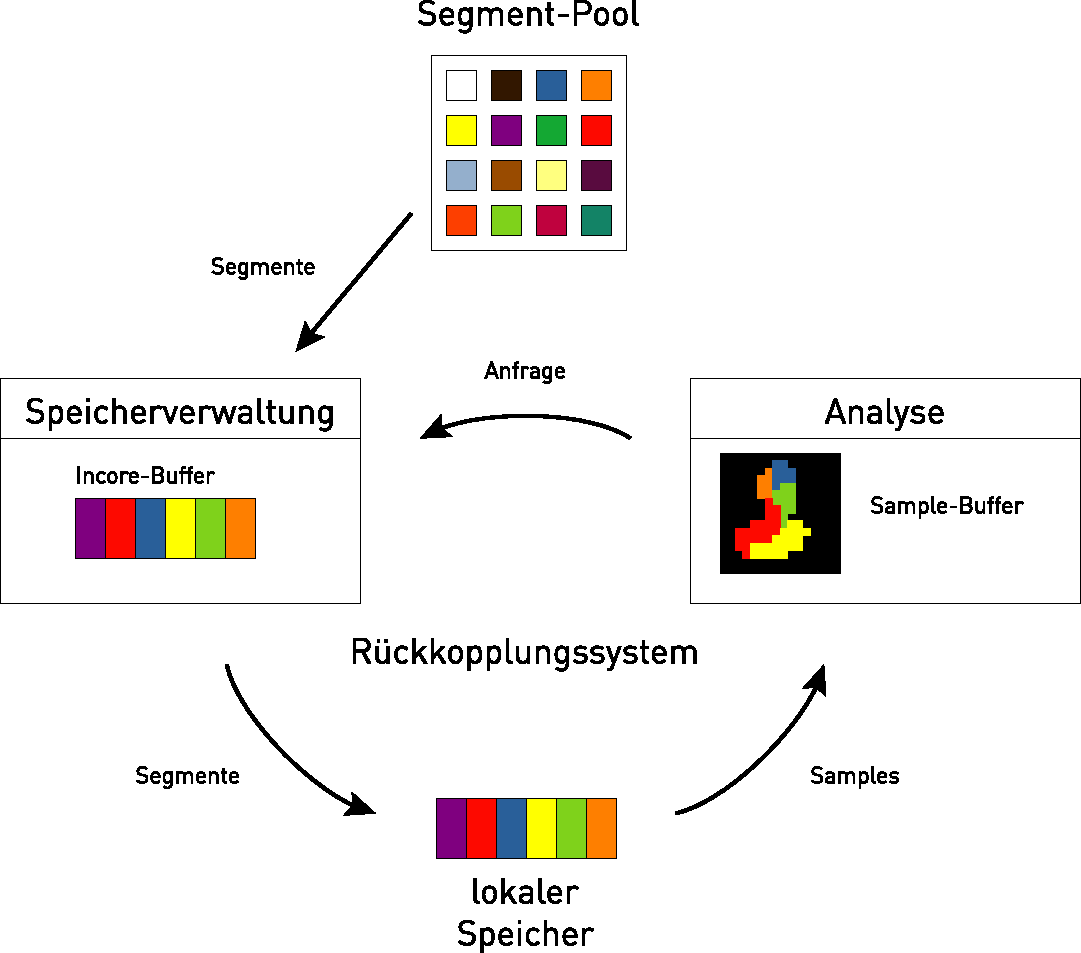
\includegraphics[width=0.75\textwidth]{out-of-core-ansatz/figures/four_part_setup.pdf}
  \caption{Schematischer Aufbau des Out-Of-Core-Systems\label{four_part_setup}}
\end{figure}

Der Incore-Buffer, der auf Client- und Serverseite Vorhanden ist, wird wie der SVO in Segmente gleicher Gr��e (\textbf{\textit{Slots}}) aufgeteilt von denen jeder ein Treelet aufnehmen kann. Die Wahl einer einheitliche Treelet- und Gr��e verhindert somit Fragmentierung des Incore-Buffer und entsprechenden Aufwand zu Defragmentierung.\\
Die Analyse arbeitet serverseitig auf den im Incore-Buffer vorhandenen Treelets.



%\newpage
\chapter{Erstellung der SVO-Struktur}


\section{Ein generalisiertes System zur SVO-Erstellung}
Das System zur Erstellung der SVO-Struktur ist modular aufgebaut und besteht prinzipiell aus drei Teilen: Dem \textbf{\textit{Build-Manager}} der den Ablauf der SVO-Generierung steuert, einem \textbf{\textit{Treelet-Builder}} der die Treelets erstellt und abh�ngig vom Typ der Eingabedaten gew�hlt wird und einem \textbf{\textit{Attributgenerator}} der Abh�ngig von Eingabedaten und gew�nschter Attributkonfiguration der Ausgabedaten gew�hlt werden kann. Mit dieser Unterteilung des Systems ist es prinzipiell m�glich verschiedenste Eingabedaten wie 3D-Objekte aus Dreiecksnetzen oder Punktwolken zu verarbeiten und eine Vielzahl von Attributtkonfigurationen zu erstellen. Durch den modularen Aufbau und der Bereitstellung entsprechender Basisklassen ist es m�glich Unterst�tzung f�r weitere Eingabeformate zu schaffen.


\section{Erzeugung der Treelet Struktur}
Die SVO-Struktur wird schon bei der Erstellung segmentiert, das hei�t, in Treelets unterteilt aufgebaut. Dies bietet die M�glichkeit bereits erzeugte Treelets auf die Festplatte auszulagern, sollte der Arbeitsspeicher nicht aussreichen um die erzeugten Daten zu halten.\\
Als Eingabe werden zun�chst die gew�nschte, minimale Tiefe des resultierenden Octrees, die Speichergr��e der Treelets und der Pfad zu den Ausgangsdaten ben�tigt. Der Build-Manager erstellt zun�chst ein initiales, leeres Treelet (\textit{Wurzel-Treelet}) und �bergibt dieses zusammen mit den Eingabeparametern und den Ausgangsdaten an den Treelet-Builder. Dieser f�llt das Treelet anhand der Eingabedaten. Dabei werden alle entstandenen Blatt-Knoten, die noch nicht die gew�nschte, minimale Tiefe in der Octree-Struktur aufweisen, notiert. Zu jedem dieser Blattknoten wird unter Anderem seine Tiefe, seine Transformation relativ zum Wurzelknoten und eine Liste der Primitive der Ausgangsdaten gespeichert, die in diesem Blattknoten liegen. Ausserdem wird jeweils der Treelet-Index, der Index des Blattknotens und dessen Elternknotens gespeichert um die Verkn�pfung der folgenden Treelets realisieren zu k�nnen (vgl. Segmentierung !!!).\\
Der Build-Manager speichert diese Informationen in einer Queue und erzeugt f�r jeden Eintrag ein neues Treelet (\textit{Top-Down}). Diese werden durch die gespeicherten Treelet- und Blattknotenindices des Wurzel-Treelets initialisiert und sind so logisch mit diesem verbunden. Jedes dieser Treelets wird wiederum dem Treelet-Builder �bergeben, der sie anhand der jeweiligen Untermenge der Primitive und der gespeicherten Transformation des zugrundeliegenden Blatt\-knotens f�llt.\\
Der Build-Manager erzeugt sukzessiv weitere Treelets f�r alle Blattknoten bereits erstellter Treelets bis die geforderte minimale Tiefe des Octrees f�r alle Blattknoten erreicht ist. F�r Blattknoten die diese Tiefe erreicht haben, erzeugt ein Attributgenerator anhand deren Transformation und Primitivliste die gew�nschten Attribute. Die Liste der jeweils beteiligten Primitive und alle weiteren Informationen die zur Erstellung weiterer Treelets ben�tigt w�rden k�nnen an dieser Stelle gel�scht werden.\\
Ist die Erstellung der Treelets abgeschlossen werden die Attribute der inneren Knoten durch Mitteln der Attribute ihrer Untergeordneten Knoten erstellt. Dies geschiet f�r alle Treelets in umgekehrter Reihenfolge ihrer Erstellung (\textit{Bottom-Up}). So wird sichergestellt, dass der Wurzelknoten eines Untergeordneten Treelets bereits Attributinformation enth�lt wenn sein �bergeordnetes Treelet diese zur Generierung seiner Attribute in seinen Blattknoten ben�tigt.\\
Ist die Erstellung der Attribute bis in den Wurzelknoten des Wurzel-Treelets vorangeschritten ist die Erstellung des Octrees abgeschlossen. 


\section{Arbeitsweise des Treelet-Builders}
Der Treelet-Builder erstellt die Knoten in der Breite (\textit{Breadth-First}) und arbeitet daher intern auf einem FIFO-Kontainer (\textit{Queue}). Der Aufbau eines Elementes dieses Queue ist im Listing \ref{lst:queueelement} zu sehen. Jedes Element der Queue entspricht einem Knoten in der SVO-Struktur und enth�lt einerseits alle Informationen die n�tig sind diesen Knoten seinem �bergeordneten Knoten mitzuteilen und andererseits die Erzeugung weiterer Unterknoten zu erm�glichen.
\begin{lstlisting}[caption={Queue-Element},label={lst:queueelement}]
struct QueueElement
{
  // Knoten-Index des Knotens innerhalb des Treelets
  unsigned              _localLeafIndex;         
  // Kind-Index des Knotens innerhalb seines Eltern-Knotens
  char                  _idx;                    
  // Knoten-Index des Eltern-Knotens
  unsigned              _parentLocalNodeIndex;   
  // Tiefe des Knotens in der SVO-Struktur
  unsigned              _depth;                  
  // Transformation des Knotens relativ zum Wurzelknoten
  gloost::Matrix        _aabbTransform;          
  // In diesem Knoten enthaltene Primitive der Ausgangsdaten
  std::vector<unsigned> _primitiveIds;           
};
\end{lstlisting}
Initial wird ein Queue-Element stellvertretend f�r den Wurzelknoten des aktuellen Treelets erstellt. Dieses enh�lt die relative Transformation dieses Knotens in der SVO-Struktur sowie alle Primitive die in diesen Knoten fallen. F�r jeden potentiellen Kind-Knoten wird ein Queue-Element mit entsprechenden Parametern erzeugt und dessen \textit{Bounding Box} mit den Primitiven des aktuellen Queue-Elementes zum Schnitt gebracht. Dabei wird f�r jedes Kind die Untermenge an Primitiven notiert die geschnitten wurden. Falls ein Kind keine Primitive enth�lt, wird es verworfen. Die restlichen Kinder bekommen aufeinanderfolgende Positionen innerhalb des aktuellen Treelets. Der \textit{First-Child-Index} des Knotens des aktuellen Queue-Elementes wird daraufhin auf die Position des ersten Kindes gesetzt. Die Queue-Elemente der Kinder werden nun in die Queue eingereiht.\\
Vor dem Abarbeiten eines Queue-Elementes wird �berpr�ft, ob noch gen�gend freie Pl�tze f�r die maximal m�gliche Anzahl f�r Unterteilungen in Kind-Knoten im Treelet vorhanden sind. Sind also weniger als acht freie Pl�tze verf�gbar gilt das Treelet als voll. 
Ist dies der Fall werden die in der Queue enthaltenen Elemente, nach ihrer Tiefe in der SVO-Struktur, in finale und weiter zu unterteilende Elemente getrennt und in zwei Kontainern im Treelet gespeichert. Nachdem die finalen Knoten in ihren Eltern-Knoten als solche markiert wurden, wird das Treelet an den Build-Manager zur�ckgegeben.\\
Der Build-Manager erzeugt f�r jedes nicht finale Queue-Element ein weiteres Treelet. Der Index jedes Treelets wird im \textit{First-Child-Index} des zugeh�rigen Blattknotens im �bergeordneten Treelet gespeichert. Dann werden die Treelets entsprechned parametrisiert in einer eigenen Queue eingereiht um sie in entsprechender Reihenvolge an den Treelet-Builder weitergeben zu k�nnen. Der oben beschriebene Ablauf wiederholt sich daraufhin f�r jedes Treelet in der Queue. Liefert der Treelet-Builder nur noch Treelets mit finalen Blattknoten, leert sich die Queue und das Erstellen der SVO-Struktur ist abgeschlossen. 


\section{Attribut-Generation}
Zu jedem Treelet werden parallel ein oder mehrere Buffer mit verschachtelten (\textit{interleaved}) Attributinformationen erstellt (!!! BILD interleaved Attributes). Anzahl und Layout der Attribut-Buffer sind abh�ngig vom gew�hlten Attribut-Generator.\\
F�r jeden finalen Blatt-Knoten wird mit Hilfe der gespeicherten Primitiven und Transformation eine Menge von Attributen erzeugt. Dieser Vorgang soll im Folgenden anhand von Dreiecksprimitiven erl�utert werden. F�r jedes Dreieck innerhalb eines Blatt-Knotens wird ein Strahl erzeugt, der durch die Voxelmitte und senkrecht zum Dreieck verl�uft (!!! siehe Hennings grafik). Nun kann jeweils eine UV-Koordinate ermittelt werden indem der Strahl mit dem jeweiligen Dreick geschnitten wird. Durch die Wahl der Richtung ist gew�hrleistet, dass der Winkel zwischen Strahl und Dreicksnormale maximal ist, so dass die Wahrscheinlichkeit eines Schnittes erh�ht wird. Trotzdem ist es m�glich, dass der Strahl das Dreieck verfehlt, da das Dreick den Voxel beispielsweise nur in einer Ecke schneidet. Dabei treten f�r U und V Werte auf, die negativ oder gr��er als eins sind. In diesem Fall werden die Werte k�nstlich auf den zul�ssigen Bereich beschr�nkt. Dieser Trick erzeugt ein Rauschen in den Daten das aber angesichts der geringen Gr��e der Blatt-Knoten und des daraus resultierenden geringen Fehlers nicht sichtbar ist.\\
Mit Hilfe der ermittelten UV-Koordinaten k�nnen nun Attribute wie Farbe, Normale oder Texturekoordinate aus den Vertexattributen des Dreiecks trilinear interpoliert werden. Die erhaltenen Werte werden �ber alle am Voxel beteiligten Dreiecke hinweg gemittelt.  
Die daraus resultierenden Farb- und Normalenwerte werden auf 8 bit pro Komponente quantisiert bevor sie in den Attributbuffer gespeichert werden. 







%\newpage
\chapter{Sichtabh�ngige Ver�nderung des Octrees}

\section{�bersicht} 

Der Incore-Buffer wird zun�chst mit dem Wurzel-Treelet im ersten Slot initialisiert. Die adaptive Anpassung der Baumestruktur wird in vier Schritten realisiert: Zun�chst wird der Octree aus der Sicht der Kamera in den Feedback-Buffer gerendert (\textit{Analyse-Pass}). Nach diesem Schritt enth�lt dieses Buffer f�r jeden Strahl u.A. die Position des getroffenen Knoten im Incore-Buffer und einen Fehlerwert. War der getroffene Knoten ein Blatt, zu dessen Verfeinerung ein Treelet vorhanden ist, wird zus�tzlich noch dessen Index gespeichert.\\
Nach der �bertragung des Feedback-Buffers in den Hauptspeicher werden dessen Eintr�ge in zwei Kontainer verarbeitet (\textit{Vorsortierung}). Der eine enth�lt die Treelet-Indices aller Knoten die getroffen wurden und zus�tzlich die Treelet-Indices ihrer �bergeordneten Treelets bis zum Wurzel-Treelet. Der andere Kontainer enh�lt Anfragen nach Verfeinerung in Form der Treelet-Indices der anzuh�ngen Treelets. Die Fehlerinformation bleibt dabei in beiden Kontainern erhalten.\\
Jetzt werden beide Kontainer dem Speichermanagement �bergeben (\textit{clientseitige Aktualisierung}). Dort werden zun�chst die Sichtbarkeitsinformation aller im letzten Zyklus gesehenden Treelets aktuallisiert. Danach werden die neu anzuh�ngenden Treelets in den clientseitigen Incore-Buffer eingepflegt. Dabei werden nicht sichtbare Treelets entfernt falls im Incore-Buffer keine freien \textit{Slots} mehr zur Verf�gung stehen. Ge�nderte Slots werden markiert. Abschlie�end werden die ver�nderten Bereiche des Incore-Buffers an den Server �bertragen und stehen nun dem Renderer f�r den n�chsten Zyklus zur Verf�gung (\textit{serverseitige Aktualisierung}).\\
Die folgenden Abschnitte werden diese Schritte genauer betrachten.

\section{Der Analyse Pass}
Um die Last die durch diesen zus�tzlichen Render-Pass entsteht m�glichst gerring zu halten ist die Gr��e des zur Analyse verwendeten Zielbuffer wesentlich kleiner als die des f�r die Bildgenerierung verwendete Frame-Buffers. Um Artefaktbildung zu vermindern werden die Strahlen bei jedem Analyseschritt durch Zufallswerte parallel zur Sicht-Ebene verschoben. Die Verschiebung ist dabei so gew�hlt das �ber die Zeit im Bereich von $nxn$ Frame-Buffer Texeln abgetasted wird wobei $n$ das Verh�ltnis der Gr��en von Frame-Buffer und Analyse-Buffer ist.
Damit ist es m�glich den Analyse-Buffer auf bis $1/8$ der G��e des Frame-Buffers zu verkleinert ohne das es durch Aliasing zu Artefaktbildung kommt oder zu wenig Information zur Verf�gung steht um die nachfolgende dynamische Anpassung des Octrees zu treiben.\\

Das F�llen des Feedback-Buffers erfolgt analog zum bilderzeugenden Raycasting in OpenCl. Nach der Traversierung des Octrees liegt f�r jeden Strahl eines der folgenden drei Ergebnisse vor:  
\begin{enumerate}
  \item der Strahl trifft nicht  
  \item der Strahl trifft einen inneren Knoten
  \item der Strahl trifft ein Blatt
\end{enumerate}
Im ersten Fall wird nichts zur�ckgegeben, im Zweiten nur die Position des Voxels im Incore-Buffer und die L�nge des Strahles. Im dritten Fall wird zus�tzlich der Verweis auf ein evt. vorhandenes Sub-Treelet und die Differenz zwischen vorgefundener Voxelgr��e und der f�r die L�nge des Strahles idealen Voxelgr��e als Fehlerwert gespeichert.

\begin{lstlisting}[caption=Struktur eines Feedback-Elementes]{structFeedBackDataElement}
  struct FeedBackDataElement
  {
    int   _nodeId;
    float _error;
    int   _subTreeletGid;
    float _tmin;
  };
\end{lstlisting}


\section{Vorsortierung}
Nach dem Transfer des Analyse-Buffers vom Server in den Hauptspeicher, werden dessen Elemente ausgewertet. Dabei werden zwei Kontainer mit unterschiedlichen Sichtinformationen gef�hlt. Im ersten Kontainer werden Indices von Treelets notiert, die bereits im Incore-Buffer vorhanden sind, im Zweiten nur Anfragen nach neuen Treelets. Beide Kontainer sind nach dem Fehlerwert der Eintr�ge absteigend sortiert wobei jeder Treelet-Index �ber beide Kontainer hinweg unique ist.\\
Im oben beschriebenen Fall 1 (der Strahl trifft nicht) liegen keine Sichtbarkeitsinformation vor weshalb solche Eintr�ge �bersprungen werden. Im Fall 2 (der Strahl trifft einen inneren Knoten) wird �ber die erhaltene Position des Knoten im Incore-Buffer und �ber die Gr��e eines Treelets auf den \textit{Slot} des zugeh�rigen Treelets und damit auch auf den entsprechenden Treelet selbst geschlossen. Durch die in den Treelets gespeicherten Eltern-Information werden zus�tzlich alle �bergeordneten Treelets als sichtbar notiert. Tritt bei der Notation ein Treelet mehrfach auf, wird jeweils der gr��te Fehler notiert.\\
Im Fall 3 (der Strahl trifft ein Blatt) wird f�r den Blattknotenindex wie im Fall 2 vorgegangen. Zus�tzlich wird der Treelet-Index des anzuh�ngenden Treelets im entsprechenden Kontainer gespeichert. Tritt ein Treelet-Index mehrfach auf wird auch hier nur ein Eintrag mit dem gr��ten Fehler gespeichert.\\
Nachdem alle Elemente des Feedback-Buffers verarbeitet wurden werden beide Kontainer dem Speichermanager �bergeben.

\section{Clientseitige Aktualisierung}
Die Pflege der Sichtbarkeitsinformationen der bereits im Incore-Buffer befindlichen Treelets ist trivial: Zun�chst wird die Sichtbarkeit jedes \textit{Slots}, d.h. die Sichtbarkeit jedes im \textit{Incore-Buffer} befindlichen Treelets dekrementiert. Dann wird die Sichtbarkeit derjenigen Treelets aktualisiert, die beim letzten Analyse-Pass gesehen wurden. Dabei wird die Sichtbarkeit auf einen vorher festgelegten Maximalwert gesetzt der dem Gr��enverh�ltnis von Render-Buffer und Analyse-Buffer entspricht. %Da die Anzahl der berechneten Samples im Analyse-Buffer bei einem Gr��enverh�ltnis von $1/8$ nur einem $1/64$ der berechneten Pixel im Framebuffer entspricht w�hre anzunehemen das die miximale Sichtbarkeitswert h�her sein m�sste. 

\subsection{Einf�gen eines Treelets}
F�r das Einf�gen eines Treelts aus dem in der Vorsortierung erstellten Kontainers wird zun�chst ein freier Slot innerhalb des Incore-Buffers ben�tigt. Ist dieser vorhanden kann das Treelet an die ensprechende Stelle im Incore-Buffer kopiert werden. Der Slot-Index wird im Treelet-Objekt gespeichert und zur Aktuallisierung des serverseitigen Incore-buffers vorgemerkt. Die folgende Ver�nderung der Baumstruktur kann in Listing \ref{lst:insert_treelet} nachvollzogen werden. Aus dem Treelet werden folgende Informationen gelesen:
\begin{enumerate}
  \item der Treelet-Index des Eltern-Treelets
  \item der Knoten-Index des Blattes, an dem das Treelet angeh�ngt werden soll
  \item der Eltern-Knoten-Index des Blattes
  \item die Position des Blattes in seinem Eltern-Knoten
\end{enumerate}
Damit wird nun die Position des ensprechneden Blattknotens des Eltern-Treelets im Incore-Buffer ermittelt und durch den Wurzelknoten des anzuh�ngenden Treelets ersetzt. Dadurch muss dessen relative Index zu seinem ersten Kindknoten angepasst werden. Der erste Kindknoten des neuen inneren Knotens findet sich immer an zweiter Position innerhalb des angeh�ngten Treelets im Incore-Buffer. Der Blattknoten wird damit zu einem inneren Knoten, was wiederum in seinem Elternknoten an der ensprechenden Stelle in der \textit{Childmask} markiert wird. In einem weiteren Kontainer wird vermerkt, dass das Parent-Treelet nun ein neues Kind-Treelet im Incore-Buffer besitzt. Abschlie�end wird der Slot-Index des Parent-Treelets zur sp�teren serverseitigen Aktualisierung vorgemerkt. 

\begin{lstlisting}[caption={Einf�gen eines Treelets},label={lst:insert_treelet}]
 ...
 Treelet* treelet = _treelets[tve._treeletGid];
 gloostId parentTreeletGid                = treelet->getParentTreeletGid();
 gloostId parentTreeletLeafPosition       = treelet->getParentTreeletLeafPosition();
 gloostId parentTreeletLeafParentPosition = treelet->getParentTreeletLeafsParentPosition();
 gloostId parentTreeletLeafIdx            = treelet->getParentTreeletLeafIdx();

 Treelet* parentTreelet = _treelets[parentTreeletGid];
 unsigned leafPositionInIncoreBuffer       = parentTreelet->getSlotGid()
                                           * _numNodesPerTreelet+parentTreeletLeafPosition;
 unsigned leafParentPositionInIncoreBuffer = parentTreelet->getSlotGid()
                                           * _numNodesPerTreelet+parentTreeletLeafParentPosition;

 // copy root node of new Treelet to the leaf of parents Treelet
 _incoreBuffer[leafPositionInIncoreBuffer] = _incoreBuffer[incoreNodePosition];

 // update leaf mask of leafs parent so that the leaf is no leaf anymore
 _incoreBuffer[leafParentPositionInIncoreBuffer].setLeafMaskFlag(parentTreeletLeafIdx, false);

 // update first child position within leaf/root (relative value within the incore buffer)
 _incoreBuffer[leafPositionInIncoreBuffer].setFirstChildIndex( (int)(incoreNodePosition+1)
                                                              -(int)leafPositionInIncoreBuffer);

 // mark incore slot of parent to be uploaded to device memory
 markIncoreSlotForUpload(parentTreelet->getSlotGid());

 // note treeletGid to parent position within the _childTreeletsInIncoreBuffer
 _childTreeletsInIncoreBuffer[parentTreeletGid].insert(tve._treeletGid);

 return true;
}
\end{lstlisting}


\subsection{Entfernen eines Treelets}
Ist f�r das Einf�gen eines Treelets kein Slot mehr verf�gbar muss zun�chst ein Slot dessen Treelet nicht sichbar war wieder frei gegeben werden. Dazu wird der Baum der Treelets in einem Thread durchsucht und eine Menge von Kandidaten f�r das Entfernen vorgehalten. Da diese Suche nebenl�ufig geschiet ist nicht sichergestellt, dass dieser Kaditat zum Zeitpunkt des Entfernens noch valide ist. Deshalb muss vor dem eigentlichen Entfernen der Sichtbarkeitswert des Slots zun�chst erneut �berpr�ft werden. Ausserdem ist es m�glich, dass zwar das entsprechende Treelet selbst nicht sichtbar war, jedoch im Falle des Entfernens der entsprechende Blatt-Knoten des Eltern-Treelts. Bild (!!!BILD EINF�GEN) illustriert diesen Fall der ausnahmslos an den R�ndern der Geometry auftritt. Im Bild befindet sich ein geladenes Treelet hinter einer konvexen W�lbung der Geometry und kann so nicht vom Analyse-Pass gesehen werden. Wird dieses Treelt jedoch entfernt, ragt der entstehende Blatt-Knoten des Eltern-Treelets �ber die W�lbung hinaus. Im n�chsten Zyklus w�rde dieses Blatt wieder verfeinert werden wodurch es zu flakernden Artefakten an den Geometriekanten kommt. Um diese Artefaktbildung zu verhindern werden Umgebungsinformationen, sprich die Sichtbarkeit des Eltern-Treelts mit�berpr�ft. Nur wenn auch das Eltern-Treelet nicht sichtbar ist, kann das Treelet sicher entfernt werden.\\
Alle Slots von im Incore-Buffer gespeicherten Treelts die sich unterhalb des zu entfernenden Treelts befinden k�nnen sofort freigegeben werden. Dazu wird die Kind-im-Incore-Buffer-Information des Kandidaten-Treelets und rekursiv die aller untergeordneten Treelets traversiert. So werden im g�nstigen Fall gleich mehrere Slots freigegeben.\\
Die Manipulation des Incore-Buffers zum Entfernen des Kandidaten-Treelets l�uft weitestgehens analog zum Einf�gen ab. Die folgenden Schritte k�nnen im Listing \ref{lst:remove_treelet} nachvollzogen werden. Wieder wird das Eltern-Treelet, die Position des entsprechenden Blatt-Knoten und dessen Eltern-Knotens ermittelt. Dann wird der Blatt-Knoten durch sein Original aus dem Eltern-Treelet �berschrieben. Aus dem inneren Knoten wird so wieder ein Blatt-Knoten mit Verweis auf ein m�gliches anh�ngbares Treelet. Dies wird im Eltern-Knoten des Blatt-Knotens an der entsprechenden Stelle in der \textit{Childmask} markiert. Da sich damit das Eltern-Treelet im Client-seitigen Incore-Buffer ge�ndert hat muss dessen Slot zur serverseitigen Aktuallisierung vorgemerkt werden.
%Ist der Incore-Buffer zu klein um den ben�tigten Schnitt durch den Baum der Treelets zu halten, stehen keine Kandidaten zum Entfernen zur Verf�gung. In diesem Fall wird f�r jedes Treelet im Incore-Buffer
\begin{lstlisting}[caption={Entfernen eines Treelets},label={lst:remove_treelet}]
  ...  
  gloostId parentTreeletGid                = treelet->getParentTreeletGid();
  gloostId parentTreeletLeafPosition       = treelet->getParentTreeletLeafPosition();
  gloostId parentTreeletLeafParentPosition = treelet->getParentTreeletLeafsParentPosition();
  gloostId parentTreeletLeafIdx            = treelet->getParentTreeletLeafIdx();

  gloost::gloostId slotGid       = treelet->getSlotGid();
  gloost::gloostId parentSlotGid = _treelets[parentTreeletGid]->getSlotGid();

  unsigned leafPositionInIncoreBuffer       = parentSlotGid
                                              *_numNodesPerTreelet + parentTreeletLeafPosition;
  unsigned leafParentPositionInIncoreBuffer = parentSlotGid
                                              *_numNodesPerTreelet + parentTreeletLeafParentPosition;

  // copy original node/leaf to incore leaf position
  _incoreBuffer[leafPositionInIncoreBuffer] = getTreelet(parentTreeletGid)->getNodeForIndex(parentTreeletLeafPosition);

  // update leaf mask of leafs parent so that the leaf is a leaf again
  _incoreBuffer[leafParentPositionInIncoreBuffer].setLeafMaskFlag(parentTreeletLeafIdx, true);

  // mark incore slot of parent to be uploaded to device memory
  markIncoreSlotForUpload(parentSlotGid);

  // clear slot info
  _slots[slotGid] = SlotInfo();

  // add slots to available/free slots
  _freeIncoreSlots.push(slotGid);

  // remove assoziation from treelet gid to slot
  treelet->setSlotGid(-1);

  _childTreeletsInIncoreBuffer[parentTreeletGid].erase(treeletGid);

  return true;
}
\end{lstlisting}


\section{Serverseitige Aktualisierung}
Die Slots die beim Einf�gen und Entfernen von Treelets markiert wurden werden in diesem Schritt auf den Server �bertragen. Dabei kann im einfachsten Fall jeder Slot innerhalb des Incore-Buffers einzeln �bertragen werden. Dies f�hrt jedoch zu vielen Einzel�bertragungen von geringer Gr��e. Dies ist sehr ung�nstig da f�r jede Kopieroperation ein nicht unerheblicher Verwaltungsaufwand innerhalb der OpenCL-API anf�llt (!!! NACHWEIS). Handelt es sich beim verwendeten Server um eine GPU m�ssen die Daten zus�tzlich �ber den PCI-Express-Bus �bertragen werden. Auch hier kann die maximale �bertragungsrate nur duch m�glichst gro�e Pakete erreicht werden (!!! NACHWEIS).\\
Um die Anzahl der Kopieraufrufe m�glichst gering zu halten werden deshalb nahe aneinanderliegende Slots zusammengefasst und gemeinsam kopiert. Dazu werden die Indices der zu aktualisierenden Slots sortiert vorgehalten. Ausgehend vom ersten Slot-Index wird der zu kopierende Speicherbereich so lange bis zum n�chsten Slot erweitern bis das Verh�ltnis zwischen zu aktualisierenden Slots und unver�nderten Slots innerhalb dieses Bereiches unter ein festgelegtes Niveau sinkt.\\
Am effizientesten arbeitet dieser Ansatz wenn der Incore-Buffer anfangs noch leer ist da die Slots-Indices aufeinanderfolgend herausgegeben werden und damit an einem St�ck auf den Server transferiert werden.
%Mit steigender Fragmentierung des Incore-Buffers sinkt die Einsparung jedoch und schwankt stark. Bei einem vorgegebenen Verh�ltis zu aktualisierenden Slots von 20\% etwa schwankt die Einsparung zwischen 10\% bis 92\% und lag �ber einen Zeitraum von 60 Sekunden im Mittel bei etwa 43\%. Die hier examplarisch genannten Werte sind jedoch wenig aussagekr�ftig, da das Verhalten des Ansatzes nicht nur von der Anzahl der Slots, der Gr��e und dem Fragmentierungsgrad des Incore-Buffers abh�ngt, sondern auch von der Geometrie und der Kameraposition �ber die Zeit. Eine Verbesserung zum einzelnen Kopieren der Slots ist jedoch erkennbar.
Das Zusammenfassen der Slots kann ausserdem in einem Thread ausgelagert werden damit sich der entstehende Zeitaufwand nicht auf die Bildrate auswirkt. \\

\section{Laufzeitbetrachtung}

\newpage
\chapter{Ergebnisse}


\section{Out-Of-Core-Ansatz}


\section{Serverseitige Aktualisierung}
Die in Abschnitt \ref{sec:serverseitige_aktualisierung} beschriebene Zusammenfassung der zu kopierenden Incore-Buffer-Slots wirkt sich deutlich auf die zum �bertragen der ge�nderten Speicherbereiche ben�tigte Zeit aus. Wie beschrieben arbeitet der Ansatz am besten wenn die zu transferierenden Speicherbereiche 
Mit steigender Fragmentierung des Incore-Buffers sinkt die Einsparung jedoch und schwankt stark. Bei einem vorgegebenen Verh�ltis zu aktualisierenden Slots von 20\% etwa schwankt die Einsparung zwischen 10\% bis 92\% und lag �ber einen Zeitraum von 60 Sekunden im Mittel bei etwa 43\%. Die hier examplarisch genannten Werte sind jedoch wenig aussagekr�ftig, da das Verhalten des Ansatzes nicht nur von der Anzahl der Slots, der Gr��e und dem Fragmentierungsgrad des Incore-Buffers abh�ngt, sondern auch von der Geometrie und der Kameraposition �ber die Zeit. Eine Verbesserung zum einzelnen Kopieren der Slots ist jedoch erkennbar.

\section{Verbesserungen}
...

%\newpage
%\input{Ausblick/Ausblick.tex}
%\newpage
%\addcontentsline{toc}{chapter}{Literatur}
%\bibliography{literatur}
%\newpage
%\input{Appendix/Appendix.tex}
\end{document}